\chapter{La sicurezza privata}
\label{capitolo2}
\thispagestyle{empty}

\begin{quotation}
	\noindent\footnotesize\emph{\textquotedblleft Giuro di osservare lealmente le leggi e le altre disposizioni vigenti nel territorio della Repubblica e di adempiere le funzioni affidatemi con coscienza e diligenza, nel rispetto dei diritti dei cittadini.\textquotedblright}
	\flushright{Giuramento di una guardia particolare giurata}
\end{quotation}
La sicurezza (dal latino "sine cura": senza preoccupazione) può essere definita come la "conoscenza che l'evoluzione di un sistema non produrrà stati indesiderati". In termini più semplici è: sapere che quello che faremo non provocherà dei danni.\cite{wiki:sicurezza}
\section{Le vigilanze private}
La vigilanza privata è l'attività, posta in essere da persone o da enti di coloro che operano nel campo della sicurezza privata, a tutela di persone, beni e/o enti pubblici o privati \cite{wiki:vigilanza}.\\
Le vigilanze private sono aziende che si occupano della protezione di persone e di beni mobili ed immobili, esse derivano direttamente dalle milizie cittadine del medioevo che, in tempo di pace svolgevano il compito di controllare e garantire la sicurezza dei cittadini durante la notte, nelle fiere e nei mercati.\\
Oggi le vigilanze private si occupano di diversi aspetti della sicurezza tramite l'utilizzo di tecnologie all'avanguardia. Tra queste attività troviamo:
\begin{description}
	\item[Piantonamento:] questo tipo di attività consiste nel presidio fisso da parte di una o più guardie particolari giurate (GPG) dotate di protezione antiproiettile e solitamente armate, esse sono collegate in modo costante con una centrale operativa. Solitamente tale attività viene svolta presso istituti di credito e enti pubblici. Possiamo distinguere tra piantonamenti diurni, piantonamenti notturni o piantonamenti per brevi periodi. Tale attività viene svolta in quei luoghi nei quali esiste un pericolo costante.
	\item[Servizio ispettivo:] questa attività consiste nell'ispezione saltuaria di alcune zone come piccole imprese, locali e aree circoscritte. Svolto principalmente durante le ore notturne consiste in una visita della zona e nell'esame degli ingressi, degli infissi e del perimetro. Se la GPG durante l'ispezione nota delle anomalie provvede a contattare la centrale operativa che effettuerà gli opportuni controlli ed avviserà eventualmente le forze dell'ordine.
	\item[Trasporto valori:] in questo caso si tratta di un servizio di scorta effettuato da personale armato e dotato di protezioni antiproiettile ed effettuato tramite l'ausilio di mezzi blindati.
	\item[Sala conta:] questa attività è destinata soprattutto agli istituti di credito e ai centri commerciali. Il denaro viene prelevato dalla sede del cliente e prima di essere custodito nel \emph{caveau} dell'istituto di vigilanza vine ricontato trattato e confezionato secondo precise istruzioni.
	\item[Localizzazione satellitare:] tramite il sistema GPS è possibile localizzare a distanza un mezzo, inoltre è possibile effettuare alcune operazioni per gestire il mezzo in tempo reale. Tale servizio è rivolto soprattutto ai possessori di auto di valore, ad aziende di trasporto, ai mezzi blindati, e a chiunque abbia necessità di tenere sotto controllo la propria flotta di veicoli. Tale servizio è possibile grazie ad un apparecchio dotato di ricevitore GPS e di un interfaccia GSM o UMTS per la comunicazione dei dati.
	\item[Teleallarme:] questo servizio consiste nell'installazione di un sistema antintrusione in abbinata ad un sistema di telecamere dove è necessario, collegati alla centrale operativa in modo da ricevere le eventuali segnalazioni di allarme e gestirle di conseguenza.
	\item[Telesoccorso:] molto simile al teleallarme ma questa volta la periferica invia le segnalazioni di allarme alla centrale solo nel caso in cui una persona prema un pulsante di allarme e non in modo automatico.
	\item[Videosorveglianza:] sistema complementare a quello di teleallarme o di telesoccorso avviene tramite l'utilizzo di telecamere collegate con la centrale operativa dell'istituto di vigilanza. Tale meccanismo permette di valutare la reale presenza di eventuali pericoli e di guidare i controlli.
\end{description}
Nella nostra trattazione ci occuperemo solo alcuni di questi servizi in particolare del teleallarme e del telesoccorso oltre ad alcune funzionalità complementari e di supporto a queste attività.
\subsection{La vigilanza di LIS}
Fondata nel 1982, LIS si contraddistingue nel panorama italiano per l'eccellente qualità dei servizi e prodotti offerti, per l'elevato standard della tecnologia usata e per la completezza dell'offerta proposta.\cite{lis:chisiamo}.\\
LIS, non si occupa di tutti gli aspetti di vigilanza visti in precedenza, si concentra, invece, su quegli aspetti che permettono agli operatori di individuare in modo rapido le minacce ed i pericoli, ed ad agire di conseguenza inviando sul posto delle guardie giurate o contattando direttamente le forze dell'ordine nei casi più gravi evitando tuttavia di contattare il cliente nei casi in cui le segnalazioni risultano non essere generate da un reale pericolo ma semplicemente da anomalie del sistema.
I servizi di LIS si concentrano perciò principalmente sul teleallarme e telesoccorso affiancati nella maggior parte dei casi da meccanismi di videosorveglianza.\\ 
A differenza della maggior parte delle vigilanze, LIS non sfrutta i normali ponti  radio per la comunicazione con le centrali di sicurezza, ma utilizza i mezzi di comunicazioni preesistenti nelle sedi da controllare in modo da avere sempre a disposizione più di un canale di comunicazione come ad esempio, linee PSTN e GSM utilizzate una come backup dell'altra; in alcuni casi più critici vengono, inoltre, installate delle periferiche di comunicazione supplementari per trasmettere eventuali guasti della centrale principale come quella mostrata in \fname{fig:webuall}
\section{Le tecnologie di LIS}
\begin{figure}
	\centering
	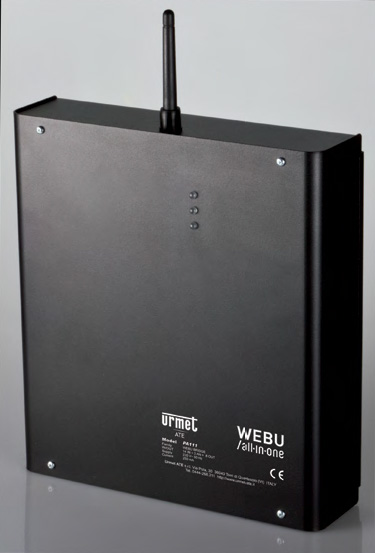
\includegraphics[width= 0.4\linewidth]{pictures/webuall.jpg}
	\caption{Foto di una Webu All-In-One}\label{fig:webuall}
\end{figure}
LIS sfrutta una serie di tecnologie innovative in tutti i settori del controllo di sicurezza, si parte dall'installazione dell'hardware dal cliente che solitamente comprende una centrale antintrusione di ultima generazione tra cui:
\begin{itemize}
	\item Tecnoalarm;
	\item UTC Fire \& Security;
	\item Bentel.
\end{itemize}
Tutte centrali che permettono la ricezione degli allarmi tramite connessioni ADSL e GPRS, ed inoltre forniscono dei software di telegestione tramite gli stessi canali di comunicazione.\\
Affiancato alla centrale antintrusione solitamente LIS installa una periferica di backup come ad esempio la \emph{Webu All-In-One} della \emph{Urmet} (\fname{fig:webuall}); questa periferica viene utilizzata come backup della centrale di d'allarme in quanto dispone di una serie di ingressi programmabili che possono essere collegati direttamente alla centrale d'allarme, inoltre, può venire utilizzata  dalle centrali più datate come ponte per il vettore PSTN. Dove possibile, inoltre, viene installato anche un sistema di videosorveglianza che permette un analisi più approfondita della situazione; in particolare, dove il budget lo permette, viene installato un sistema \emph{Dallmeier} che offre meccanismi di compressione delle registrazioni quando queste vengono consultate da remoto\cite{dallmeier:premote}.\\
Fino ad ora abbiamo analizzato l'hardware che LIS installa presso il cliente; analizziamo ora come LIS riceve e gestisce gli allarmi provenienti da questo hardware. In primo luogo, prima del nostro intervento, LIS utilizzava solo i vettori PSTN e ,solo per alcuni modelli della \emph{UTC}, il vettore GPRS. Per ricevere gli allarmi su questi vettori LIS utilizza due ricevitori, il primo chiamato \emph{System III} il quale è un sistema di ricezione allarmi su PSTN che permette di ricevere le segnalazioni tramite il protocollo Contact-ID o SIA su PSTN e quindi su linea telefonica tradizionale tramite i toni. Il secondo sistema è chiamato \emph{Osborne Hoffman LAN} e permette, tramite un protocollo proprietario, di ricevere gli allarmi sul canale GPRS per alcuni modelli della \emph{UTC Fire \& Security}.\\
Questi due ricevitori permettono la ricezione degli allarmi, i quali vengono poi gestiti tramite l'utilizzo di un programma proprietario denominato \emph{E-Pro} che permette la gestione degli allarmi presentando all'operatore le informazioni più importanti come l'anagrafica del cliente, il posizionamento del sensore che è ha generato l'evento, una segnalazione esaustiva della tipologia di allarme ed altre informazioni che possono essere utili; l'operatore una volta preso in carico una segnalazione la gestisce tramite questo software il quale in automatico genera un rapporto di gestione.
\begin{figure}
	\centering
	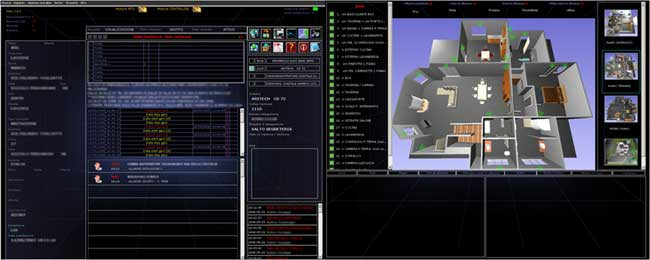
\includegraphics[width=\linewidth]{pictures/schermataepro.jpg}
	\caption{Schermata del software E-Pro}\label{fig:epro}
\end{figure}
Un esempio di schermata di gestione è mostrato in \fname{fig:epro}
\section{Terminologia utilizzata}
Prima di addentrarci nella trattazione della tesi dobbiamo fare alcune precisazioni sulla terminologia utilizzata in particolare:
\begin{description}
	\item[Centrale d'allarme:] si intende un hardware con un numero elevato di ingressi e un ridotto numero di uscite che svolge la funzione di rilevare eventuale cambiamenti di stato negli ingressi e, se il sistema è inserito, generare un allarme che può essere trasmesso tramite diversi vettori.
	\item[Zona:] sensore collegato ad un ingresso della centrale d'allarme, esso può essere di diverso tipo tra cui sensore infrarossi, volumetrico o a contatto magnetico ecc.
	\item[Partizione:] raggruppamento di diverse zone, questo raggruppamento è puramente logico ed è effettuato dalla centrale d'allarme.
	\item[Tamper:] interruttore di manomissione che fa scattare una segnalazione da parte della centrale d'allarme.
	\item[Periferica (di backup):] hardware che svolge gli stessi compiti di una centrale d'allarme tuttavia presenta un numero ridotto di contatti in ingresso e la logica è meno evoluta (non presenta la possibilità di suddividere le zone in partizioni).
	\item[Programmatore orario:] parte della logica di una centrale di allarme che effettua l'inserimento o il disinserimento dell'impianto d'allarme in modo automatico ad un determinato orario.
	\item[Ricevitore: ] sistema solitamente hardware ma a volte anche software che svolge la funzione di raccogliere e a volte tradurre in un altro linguaggio una segnalazione proveniente da una centrale d'allarme.
	\item[Centrale operativa:] luogo blindato all'interno di un istituto di vigilanza al cui interno gli operatori svolgono la funzione di ricevere e gestire segnalazioni d'allarme provenienti dalle diverse centrali d'allarme.
	\item[Inserimento:] azione eseguita su di una o più partizioni indica che le segnalazioni provenienti da dalle diverse zone appartenenti a quella partizione da quel momento generano un allarme.
	\item[Disinserimento:] azione contraria all'inserimento
	\item[Esclusione:] azione eseguita su di una zona che fa in modo che il sensore escluso non generi alcun allarme.
	\item[Inclusione:] azione contraria all'esclusione
\end{description}
\section{Cosa offre il mercato}
Al nostro arrivo in LIS la situazione presente era quella specificata in precedenza e quindi le centrali supportate erano poche, inoltre, il vettore di comunicazione principale era il PSTN. Si è quindi deciso di analizzare che cosa offrisse il mercato per valutare se sostituire il software E-Pro o aggiornarlo per renderlo più competitivo rispetto alla concorrenza.\\
Analizzeremo adesso quali sono i principali prodotti che avrebbero potuto sostituire il software di LIS analizzando in dettaglio i punti a favore e quelli a sfavore della scelta.
I software che abbiamo analizzato sono stati:
\begin{itemize}
	\item AteArgo di Urmet;
	\item WebSat Enterprise di AMA Software;
	\item Advisor Managment di UTC Fire \& Security;
	\item Mastermind e X-View di Enai.
\end{itemize}
\subsection{AteArgo}
AteArgo è un prodotto che ha alle spalle vent'anni di sviluppo da parte di \emph{Urmet}, esso si basa su un sistema Unix/Linux ed è stato il primo software per vigilanze private creato in Italia. Il continuo confronto con il mercato e l'aggiornamento tecnico costante hanno permesso di perfezionare sempre più AteArgo e adattarlo alle reali esigenze delle centrali operative degli istituti di vigilanza.\\
La centrale AteArgo è composta da due server uno principale e uno di backup con allineamento automatico dei dati in maniera trasparente all'operatore. Il software è multi-operatore e multi protocollo per quanto riguarda le segnalazioni provenienti dai vettori radio, PSTN e GSM, inoltre per alcuni prodotti sviluppati direttamente da Urmet permette anche la ricezione degli allarmi tramite vettori GPRS e TCP/IP. Il software permette di gestire delle periferiche mobili GPS per applicazioni di teleallarme come l'invio della pattuglia più vicina in caso di allarme o la verifica del servizio di ronda. Nell'ultima versione del software è possibile, tramite l'ausilio di periferiche aggiuntive, l'acquisizione video automatica dalle centrale AteArgo a seguito di un evento di allarme. Infine è possibile la gestione di sistemi video navigabili via browser.\\
Oltre a queste funzionalità il sistema è in grado di eseguire alcune funzioni automatizzate come effettuare chiamate automatiche per particolari segnalazioni effettuare il backup a caldo sia della centrale principale che quella di riserva, invio di segnalazioni direttamente al cliente tramite SMS, gestione automatica di un call-center e di un agenda cliente.\\
AteArgo fornisce anche la possibilità di rilevazioni statistiche sia in formato elettronico sia via Web. possibilità di creare report personalizzati o l'interazione con altri sistemi di centralizzazione.\\
Per quanto riguarda la gestione multi operatore ad ogni operatore viene assegnato un profilo specifico in base al suo livello di specializzazione. Per accedere al sistema ogni operatore si identifica tramite login e password con le quali attiva le funzioni a lui destinate.\\
L'interfaccia utente permette di intervenire all'arrivo di un allarme con il minor numero di azioni. Inoltre vi è un costante monitoraggio del sistema e dei collegamenti periferici.\\
Oltre a queste funzionalità di base il sistema può essere espanso tramite moduli software aggiuntivi tra cui:
\begin{description}
	\item[comunication server:] il sistema permette la comunicazione con altri sistemi informativi in modo bidirezionale assumendo la funzionalità di front-end.
	\item[Utente ricaricabile:] consente alla vigilanza di gestire clienti di tipo "ricaricabile" ovvero con la possibilità da parte del cliente di attivare o disattivare il servizio di vigilanza solamente tramite l'invio di un SMS.
	\item[Verbali:] garantisce la rintracciabilità di tutte le azioni della centrale operativa e legate ad un allarme e supporta l'operatore nella gestione degli eventi.
	\item[ArgoSound:] permette la gestione di determinate segnalazioni tramite una chiamata vocale automatica.
	\item[Fast call:] compone automaticamente un numero dalla lista dei contatti del cliente in allarme evitando errori o perdite di tempo.
	\item[Messaging:] permette alla centrale di inviare automaticamente SMS, FAX o E-Mail verso recapiti preimpostati nel caso di particolari eventi.
	\item[Modulo database:] relaziona e rende disponibili tutti i dati archiviati e permette di eseguire qualsiasi tipo di ricerca, inoltre permette di interfacciarsi con altri sistemi. Permette la creazione di indici per la stima e la valutazione degli interventi.
	\item[Modulo installatore:] questo modulo permette di sollevare l'operatore dal supervisionare una nuova installazione dando la possibilità al tecnico di collegarsi alla centrale mediante portatile o smartphone e verificare la corretta ricezione degli allarmi dell'impianto sul quale sta intervenendo.
	\item[Modulo GPS:] permette di ricevere in centrale la posizione in tempo reale del parco pattuglie e di inviare sul sito in allarme la pattuglia più vicina.
	\item[Modulo video:] permette alla postazioni operatore di collegarsi a video server e telecamere IP in tempo reale.
\end{description}
\subsection{WebSat Enterprise}
WebSat Enterprise è un software sviluppato da \emph{AMA} per la gestione di problemi di sicurezza ed emergenza degli ambienti, delle persone e dei veicoli. Esso consente la gestione di diverse tipologie di dispositivi di teleallarme come combinatori telefonici digitali (Contact-ID, SIA, Fast Format), combinatori telefonici a sintesi vocale, teleallarmi radio. Inoltre tramite l'ausilio di periferiche AMA è possibile la gestione di teleallarmi via GSM/GPRS o IP, video allarmi, video sorveglianza con telecamere IP ed anche localizzazione satellitari per il controllo delle pattuglie, dei furgoni per il trasporto valori e qualsiasi tipo di veicolo.\\
Oltre a queste caratteristiche il software \emph{WebSat Enterprise} permette un'interazione automatizzata verso il cliente tramite SMS o chiamate pre-registrate. Gestisce, inoltre, i servizi di pattuglia e di ronda tramite l'ausilio di periferiche proprietarie basate sulla tecnologia GPS. Infine permette, sempre tramite periferiche proprietarie, la gestione della videosorveglianza.\\
Per quanto riguarda l'aspetto amministrativo il software permette l'integrazione con i software amministrativi e gestionali già presenti in azienda ed è  possibile predisporre un interfacciamento per la ricezione di allarmi provenienti da altri software.\\
Il software WebSat Enterprise è:
\begin{description}
	\item [Multifunzionale:] in quanto permette all'operatore di gestire tramite un unica interfaccia sia gli allarmi provenienti da periferiche mobili sia da impianti di allarme fissi.
	\item [Geo-referenziato:] per ogni tipo di allarme sia esso fisso o mobile, vengono messe a disposizione dell'operatore il maggior numero di informazioni possibili.
	\item [Gestione delle pattuglie:] Tramite la periferica WebSat Patrol la centrale permette di gestire in modo automatizzato le pattuglie in modo da ottimizzare le pattuglie sul territorio.
	\item[Report di comunicazione verso i clienti:] la centrale è in grado di inviare avvisi di stato di allarme in modo automatico via SMS , invio automatico di report mensili, possibilità da parte del cliente di richiedere report parziali tramite l'invio di SMS.
	\item [Interfacciamento automatico con centralino telefonico:] WebSat Enterprasie consente l'automazione delle chiamate verso i contatti telefonici del cliente in caso di allarme.
	\item[Interfacciamento con altri ricevitori:] oltre ai ricevitori di AMA la Websat enterprise è in grado di interfacciarsi con tutti i ricevitori telefonici che implementano i protocolli ADEMCO 685, standard SurGuard, per ricevere gli allarmi in codice Contact ID, SIA level 2 e Ademco high Speed.
	\item [Ricezione allarmi da combinatori con sintesi vocale:] la centrale di AMA è in grado di ricevere allarmi tramite chiamate effettuate da combinatori telefonici con sintesi vocale, solamente assicurandosi che il numero del chiamante sia in chiaro.
	\item [Gestione telecamere Axis:] ad ogni sistema di teleallarme è possibile combinare una o più telecamere Axis con connessione diretta via Internet in modo da mettere a disposizione dell'operatore un sistema di videosorveglianza ad un costo contenuto.
	\item [Polling GPRS:] per quelle periferiche che sono connesse tramite canale GPRS o TCP/IP la centrale è in grado di effettuare un polling ad intervalli molto brevi per verificare l'esistenza in vita della periferica e rilevare in modo tempestivo eventuali problemi di connessione.
\end{description}
\subsection{Advisor Managment}
Advisor Managment è una soluzione di \emph{UTC Fire \& Security} pensata per centralizzare la gestione della sicurezza di uno o più siti facenti riferimento ad un unica centrale di sicurezza. Tuttavia questo prodotto non è pensato specificatamente per le vigilanze bensì per piccoli complessi residenziali o commerciali aventi un unica centrale di monitoraggio.\\
Questo sistema si concentra sulle caratteristiche necessarie alla gestione della sicurezza in ambienti particolari nel quale accedono dipendenti e lavoratori; nel quale si hanno orari di lavoro flessibili e solo la gestione integrata di controllo accessi, sicurezza antincendio e videosorveglianza permette ai security manager di avere una visione chiara e completa di tutto il sistema.\\
L'Advisor Managment offre un interfaccia intuitiva per la gestione di ambienti differenti, consente la creazione di report ed è rivolto alla gestione efficiente degli allarmi qualunque essi siano.\\
Per quanto riguarda la videosorveglianza l'Advisor Managment è in grado di supportare tutti i videoregistratori di rete TrueVison, questa integrazione permette agli operatori di avere accesso sia alle telecamere in tempo reale sia agli eventi registrati consentendo così una verifica immediata degli eventi di allarme.\\ 
L'Advisor Managment supporta le centrali antintrusione della linea Advisor Managment e Advisor Advance questo permette una gestione combinata di sistemi antintrusione e di videosorveglianza, inoltre è possibile configurare aree ad accesso limitato. Nel caso di rilevazione di un allarme, questo viene evidenziato nell'area di competenza e le immagini vengono mostrate in modo automatico all'operatore. Advisor Managment permette inoltre l'integrazione con le centrali di rilevazioni incendi della serie FP sia per il monitoraggio degli eventi sia per tutto quello che riguarda la gestione dell'impianto. Tutto questo integrato in un unico software permette di intervenire in modo tempestivo in caso di incendio; infatti, in caso di allarme la posizione del sensore viene mostrata dinamicamente e viene attivato il flusso video in tempo reale per verificare la presenza dell'incendio. Inoltre, grazie al sistema di controllo accessi è possibile sbloccare tutte le porte in modo automatico.
\subsection{Mastermind e X-View}
Mastermind è uno dei prodotti più utilizzati dalle maggiori industrie di sicurezza principalmente in US ma ultimamente anche nel resto del mondo sia nel settore privato che in quello pubblico. Questa diffusione è dovuta alla grande sicurezza e affidabilità del sistema unita alla possibilità di gestire sistemi su larga scala. I punti di forza di Mastermind sono la possibilità di lavorare sia con ambienti di piccola scala sia con ambienti più grandi. Possibilità di configurazione multi sito con ridondanza a caldo. Integrazione di molti sistemi in un unica interfaccia di sistema.\\
Mastermind è un sistema ad architettura aperta per fare in modo che i compratori possano adattare le loro tecnologie al sistema; esso permette la comunicazione tramite rete locale LAN e mette a disposizione degli SDKs per supportare al meglio lo sviluppo da parte di venditori di terze parti. come vendor di videosorveglianza.\\
Il sistema si suddivide in due parti slegate, una parte tratta il monitoring degli allarmi, l'altra parte, denominata \emph{business suite} si occupa del contatto e della gestione del cliente. Tutte queste funzioni sono supportate da una serie di applicazioni che permettono una gestione ottimale del sistema come il MASVideo che permette di registrare sui server le immagini associate ad un allarme o il MASWeb utilizzato per consentire un accesso remoto alla reportistica a clienti con particolari esigenze. Oppure X-View un software affiancato a MasterMind che permette all'operatore di costruire la propria interfaccia personale e mette a disposizione maggiori informazioni come la localizzazione GPS o la piantina dell'edificio.\\
A differenza degli altri prodotti analizzati mastermind risponde alle esigenze impostate dal cliente tramite l'utilizzo di workflows che gestiscono tutti gli eventi in modo tale da guidare l'operatore lungo una sequenza predefinita di operazioni. Inoltre questo meccanismo permette di gestire in modo automatico le operazioni più semplici e che non richiedono la necessità dell'interazione con l'operatore.\\
La parte di \emph{business suite} comprende tre sotto sezioni, la prima per definire le promozioni ed i prezzi da applicare ai clienti e organizza gli appuntamenti per le vendite. La seconda parte si occupa della relazione col cliente contenendo i dati del contratto la fatturazione dei servizi e il controllo dei pagamenti. l'ultima parte invece si occupa dell'organizzazione dell'installazione e dell'attivazione del servizio, si può occupare della gestione del magazzino mantenendo un inventario aggiornato.
Le funzionalità di Mastermind sono:
\begin{description}
	\item[VRT/IVR] ovvero la possibilità di sfruttare un centralino automatico che risponde alle richieste più comuni dei clienti senza tenere occupato inutilmente un operatore di centrale, inoltre questa funzionalità può essere sfruttata per creare chiamate automatizzate verso il cliente nel caso di allarmi specifici.
	\item[Voice Recorder Integration:] tutte le chiamate in entrata ed in uscita possono essere registrate e immagazzinate per un successivo controllo sia da parte del cliente che da parte della vigilanza nel caso in cui sia necessaria una verifica.
	\item[Report Server:] questa funzionalità permette l'invio di email o messaggi periodici con il riassunto degli allarmi e degli interventi.
	\item[MASWeb:] questa funzionalità permette ai clienti e ai tecnici di accedere alle loro informazioni per generare report o modificare i dati. Le pagine web sono strutturate per includere i servizi di monitor e reportistica, l'elenco dei servizi e le informazioni di fatturazione. I tecnici possono modificare uno stato dell'impianto e inserirlo in modalità test per ricevere sul proprio browser o sull'app l'esito dei test effettuati durante una manutenzione o installazione.
	\item[MASmobile:] questa app permette di controllare lo stato del sistema effettuare controllare lo storico eventi, agli installatori permette di mettere il sistema in modalità test per ricevere gli esiti.
	\item[Controllo accessi:] è possibile integrare la ricezione degli allarmi con sistemi di controllo accessi 
\end{description}
\subsection{La decisione}
Riassumiamo ora in \tablename~\ref{tab:riassunto} le caratteristiche dei diversi prodotti analizzati confrontandoli con il software già a disposizione di LIS.
\begin{sidewaystable}
	\begin{tabularx}{\textheight}{|p{0.11\textheight}|p{0.2\textheight}|p{0.15\textheight}|p{0.15\textheight}|p{0.15\textheight}|X|}
		\hline
		\textbf{Prodotto} & \textbf{Ricezione\newline TCP/IP e GPRS} & \textbf{Protocollo\newline TCP/IP} & \textbf{Telegestione} & \textbf{Tipo\newline connessione} & \textbf{Interfaccia grafica}\\
		\hline
		\textbf{AteArgo} & Solo periferiche proprietarie & Proprietario &  Solo per le periferiche proprietarie & Remota  &  Complicata e difficilmente usabile \\ \hline
		\textbf{WebSat} & Solo periferiche proprietarie & Proprietario & NO &  Remota &  Incentrata sulla cartografia non sul singolo sito \\ \hline
		\textbf{Advisor Managment} & Solo periferiche proprietarie & Proprietario & SI  & Locale  & Non adatto a gestire più siti \\ \hline
		\textbf{Mastermind} & SI & Standard e proprietari delle singole aziende & NO & Remota &  Completamente personalizzabile \\ \hline
		\textbf{E-Pro} & Solo UTC & Proprietari delle singole aziende & NO & Remota & Adattata negli anni alle esigenze di LIS \\ \hline
		
	\end{tabularx}
	\caption{Caratteristiche dei prodotti attualmente in commercio}\label{tab:riassunto}
\end{sidewaystable}
Come notiamo dalla tabella il software Mastermind sarebbe stato adatto alle esigenze di LIS tuttavia due motivi ci hanno spinto a continuare lo sviluppo del software E-Pro il primo è stato un fattore economico in quanto il software Mastermind per funzionare appieno necessita di una serie di hardware di supporto che avrebbe dovuto sostituire in toto quello già utilizzato da LIS, il secondo era invece più pratico in quanto gli operatori di centrale si erano abituati ad utilizzare E-Pro negli anni e riformare completamente gli operatori avrebbe richiesto parecchio tempo e probabilmente notevoli disservizi. Si è deciso perciò di proseguire con il software già presente in LIS.